% 固定来源第1页Q10，题干续于第2页。忠实保留标号/中点/隐藏边。
% u=(.7,-.5), v=(1.4,.3), h=(0,1.8)仅为平行投影基向量，非实际长度。
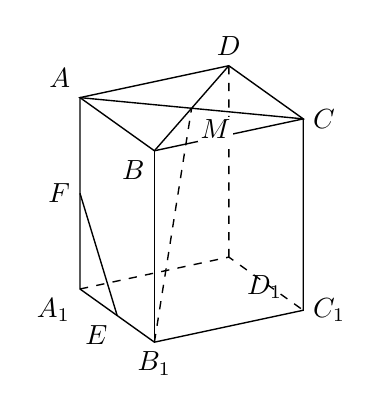
\begin{tikzpicture}[line width=.5pt,scale=1.35]
  \coordinate (A1) at (0,0);
  \coordinate (B1) at (.7,-.5);
  \coordinate (C1) at (2.1,-.2);
  \coordinate (D1) at (1.4,.3);
  \coordinate (A) at (0,1.8);
  \coordinate (B) at (.7,1.3);
  \coordinate (C) at (2.1,1.6);
  \coordinate (D) at (1.4,2.1);
  \coordinate (E) at (.35,-.25);
  \coordinate (F) at (0,.9);
  \coordinate (M) at (1.05,1.7);
  \draw (A)--(B)--(C)--(D)--cycle;
  \draw (A)--(A1)--(B1)--(C1)--(C);
  \draw (B)--(B1);
  \draw[dashed] (A1)--(D1)--(C1) (D1)--(D);
  \draw (A)--(C) (B)--(D) (E)--(F);
  \draw[dashed] (B1)--(M);
  \node[above left] at (A) {$A$};
  \node[below left] at (B) {$B$};
  \node[right] at (C) {$C$};
  \node[above] at (D) {$D$};
  \node[below left] at (A1) {$A_1$};
  \node[below] at (B1) {$B_1$};
  \node[right] at (C1) {$C_1$};
  \node[below right,xshift=3pt,yshift=-3pt] at (D1) {$D_1$};
  \node[below left] at (E) {$E$};
  \node[left] at (F) {$F$};
  \node[below right,inner sep=1pt,xshift=2pt,yshift=-3pt,fill=white] at (M) {$M$};
\end{tikzpicture}
